% !TeX document-id = {6de14b61-2d85-4533-aab5-47279ef7f4fb}
% !TeX TXS-program:compile = txs:///xelatex/[--shell-escape]
\documentclass[10pt]{beamer}

\usetheme[progressbar=frametitle]{metropolis}

\definecolor{MainColor}{RGB}{4, 104, 215}
\definecolor{SecondaryColor}{RGB}{4, 36, 73}

% \colorlet{mDarkTeal}{MainColor}
% \definecolor{mDarkTeal}{HTML}{23373b}

\setbeamercolor{title separator}{bg=MainColor,fg=MainColor}
\setbeamercolor{progress bar}{bg=SecondaryColor,fg=MainColor}
\setbeamercolor{palette primary}{bg=MainColor}
\metroset{block=fill}

\usepackage[export]{adjustbox}
\usepackage{appendixnumberbeamer}
\usepackage{booktabs}
\usepackage[scale=2]{ccicons}
\usepackage{pgfplots}
\usepackage{xspace}
\usepackage{hyperref}
\usepackage{geometry}
\usepackage{bookmark}
\usepackage{minted}


\title{Workshop\\Introduction to App Development}
\subtitle{A shallow dive into the world of App Development and Flutter\texorpdfstring{\\ \footnotesize\url{https://github.com/NEEECFEUP/WS-App-Development/}}{}}
\institute{NEEEC - FEUP}

\date{November 2022}
\author{André Campanhã}

\logo{
\includegraphics[height=1.5cm]{images/logo_oficial_bordo_c.png}}

\usepgfplotslibrary{dateplot}

\hypersetup{
  colorlinks=true,
  linkcolor=MainColor,
  filecolor=magenta,      
  urlcolor=MainColor
}

\begin{document}

\begin{frame}
  \maketitle
\end{frame}

{
    \metroset{sectionpage=none}
    \section*{Introduction}
}
\begin{frame}{Introduction}
    \begin{columns}
        \begin{column}{0.5\textwidth}
            \begin{figure}[h]
                \centering
                
\includegraphics[width=0.5\textwidth]{images/flutter.pdf}
            \end{figure}
        \end{column}
        \begin{column}{0.5\textwidth}
            \begin{figure}[h]
                \centering
                
\includegraphics[width=0.5\textwidth]{images/dart.pdf}
            \end{figure}
        \end{column}
    \end{columns}

    \vspace{4ex}

    \begin{itemize}
        \item Mobile framework for creating native(ish)\footnotemark[1] apps for Mobile (Android, iOS), Desktop (Win, Mac, Linux), Web, and Embedded
        \item Write once (dart), run everywhere(ish)\footnotemark[1]
    \end{itemize}

    \footnotetext[1]{Flutter can access native API calls via native platform code (i.e. Android SDK). This can be somewhat abstracted by using cross-platform dart packages.}
    
\end{frame}

\begin{frame}{Prerequisites}
    \begin{itemize}
        \item Programming basics (OOP familiarity recommended)
        \item Having followed Flutter's installation steps sent by e-mail
        \begin{itemize}
            \item \href{https://docs.flutter.dev/get-started/install}{Install Flutter} (Get the Flutter SDK and Android Setup)
            \item \href{https://docs.flutter.dev/get-started/editor}{Set up an editor} (Recommended: VS Code)
        \end{itemize}
    \end{itemize}
\end{frame}

{
    \metroset{sectionpage=none}
    \section*{Outline}
    \begin{frame}<beamer>
        \frametitle{Outline}
        \tableofcontents[subsectionstyle=show/hide/hide]
    \end{frame}
}
\section{Basics}

\subsection{What is a widget?}

\begin{frame}{Everything is a widget}
    The core of Flutter's layout mechanism is widgets.

    They describe what their view should look like given their current configuration and state.

    When a widget's state changes, the widget rebuilds its description, which the framework diffs against the previous description in order to determine the minimal changes needed in the underlying render tree to transition from one state to the next.
\end{frame}

\begin{frame}{Everything is a widget}
    How many widgets here?
    \begin{figure}[h]
        
\includegraphics[width=0.4\textwidth]{images/lakes-icons.png}<1->
    \end{figure}

    \begin{figure}[h]
        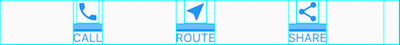
\includegraphics[width=0.4\textwidth]{images/lakes-icons-visual.png}<2->
    \end{figure}

    \only<3->{14 widgets!}
\end{frame}

\begin{frame}{Everything is a widget}
    \begin{figure}[h]
        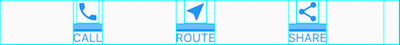
\includegraphics[width=0.4\textwidth]{images/lakes-icons-visual.png}
    \end{figure}
    \begin{figure}[h]
        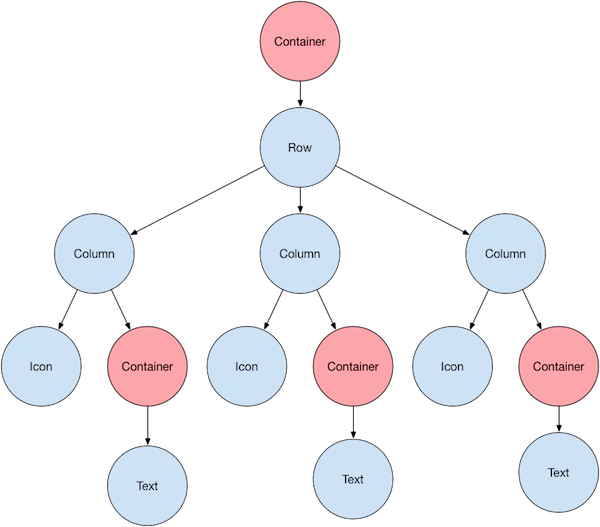
\includegraphics[width=0.6\textwidth]{images/sample-flutter-layout.png}
    \end{figure}
\end{frame}

\subsection{What is State?}

\begin{frame}{What is State?}
    \begin{block}{State}
        Information that can be read synchronously when the widget is built and might change during the lifetime of the widget.
    \end{block}
\end{frame}

\subsection{Types of widgets}
\begin{frame}{Types of widgets}

There are 2 types of widgets:

\begin{block}{Stateless Widgets}<2>
    They do not own a mutable state.

    Useful when the part of the user interface you are describing does not depend on anything other than the configuration information in the object itself and the context in which the widget is inflated.
\end{block}
    
\end{frame}

\begin{frame}{Types of widgets}
    
    There are 2 types of widgets:
    
    \begin{block}{Stateful Widgets}
        They are themselves immutable. However, they own a State.
        
        Useful when the part of the user interface you are describing can change dynamically, e.g. due to having an internal clock-driven state or depending on some system state
    \end{block}
    
\end{frame}

\subsection{Widget Lifecycle}
\begin{frame}{Widget Lifecycle}
    \begin{figure}[h]
        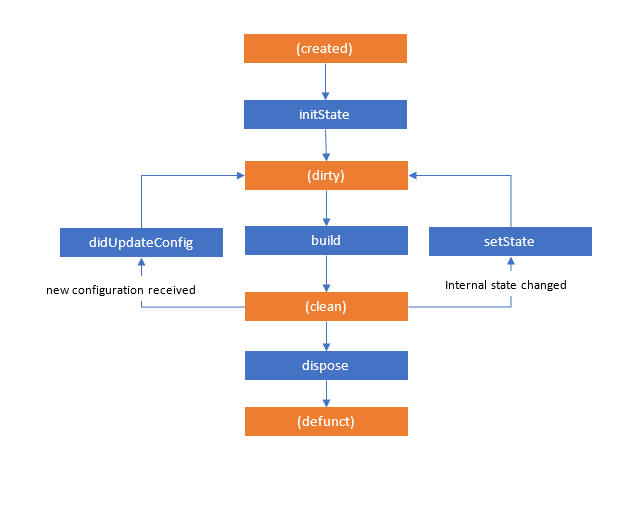
\includegraphics[width=0.8\textwidth]{images/lifecycle.png}
    \end{figure}
\end{frame}
\section{Widgets}

\begin{frame}[containsverbatim]{Container}

  \begin{figure}[h]
    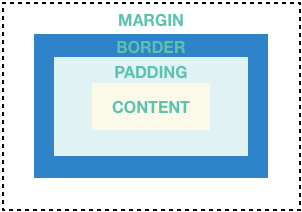
\includegraphics[width=0.25\textwidth]{images/margin-padding-border.png}
  \end{figure}

  \begin{minted}[fontsize=\footnotesize]{dart}
Container(
  margin: const EdgeInsets.all(10.0),
  color: Colors.amber[600],
  width: 48.0,
  height: 48.0,
);
	\end{minted}
  \footnotesize
  \url{https://api.flutter.dev/flutter/widgets/Container-class.html}
\end{frame}


\begin{frame}[containsverbatim]{Row}

  \begin{figure}[h]
    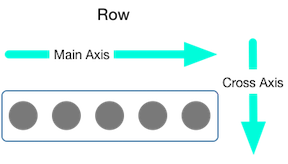
\includegraphics[width=0.25\textwidth]{images/row-diagram.png}
  \end{figure}

  \begin{minted}[fontsize=\footnotesize]{dart}
Row(
  mainAxisAlignment: MainAxisAlignment.spaceEvenly,
  children: [
    Image.asset('images/pic1.jpg'),
    Image.asset('images/pic2.jpg'),
    Image.asset('images/pic3.jpg'),
  ],
);
  \end{minted}
  \footnotesize
  \url{https://api.flutter.dev/flutter/widgets/Row-class.html}
\end{frame}

\begin{frame}[containsverbatim]{Column}

  \begin{figure}[h]
    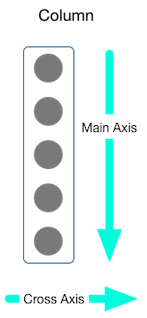
\includegraphics[height=0.25\textwidth]{images/column-diagram.png}
  \end{figure}

  \begin{minted}[fontsize=\footnotesize]{dart}
Column(
  mainAxisAlignment: MainAxisAlignment.spaceEvenly,
  children: [
    Image.asset('images/pic1.jpg'),
    Image.asset('images/pic2.jpg'),
    Image.asset('images/pic3.jpg'),
  ],
);
  \end{minted}
  \footnotesize
  \url{https://api.flutter.dev/flutter/widgets/Column-class.html}
\end{frame}

\begin{frame}[containsverbatim]{Text}

  \begin{minted}[fontsize=\footnotesize]{dart}
Text(
  'Hello, $_name! How are you?',
  textAlign: TextAlign.center,
  overflow: TextOverflow.ellipsis,
  style: const TextStyle(fontWeight: FontWeight.bold),
);
	\end{minted}
  \footnotesize
  \url{https://api.flutter.dev/flutter/widgets/Text-class.html}
\end{frame}

\begin{frame}[containsverbatim]{Elevated Button}

  \begin{minted}[fontsize=\footnotesize]{dart}
ElevatedButton(
  style: style,
  onPressed: () {print("Hello")},
  child: const Text('Click me'),
),
	\end{minted}
  \footnotesize
  \url{https://api.flutter.dev/flutter/material/ElevatedButton-class.html}
\end{frame}

\begin{frame}
  Now that we got that covered...
\end{frame}
{
  \logo{
\includegraphics[height=1.5cm]{images/logo_oficial_branco_c.png}}
  \begin{frame}[standout]
    What are we going to build today?
  \end{frame}
}
\section{Task 1 - Basic layout}

\begin{frame}{Task 1 - Basic Layout}
    If you haven't, get the source code from the \href{https://github.com/NEEECFEUP/WS-App-Development/}{Github Repository}.

    \begin{block}{Hint!}
        To print to the terminal, use:
        
        \mint{dart}| import 'dart:developer' as developer;|

        and

        \mint{dart}| developer.log('Hello!', name: 'app.log');|
    \end{block}
\end{frame}

\begin{frame}{Task 1 - Basic Layout}
    \begin{itemize}
        \item Create a screen with a Text "Hello World"
        \item A button "Click" under it
        \item When you click the button, print something to the terminal
    \end{itemize}
\end{frame}

\begin{frame}{Task 1 - Basic Layout}
    \begin{figure}[h]
        {
            \setlength{\fboxsep}{0pt}%
            \setlength{\fboxrule}{0.5pt}%
            \fbox{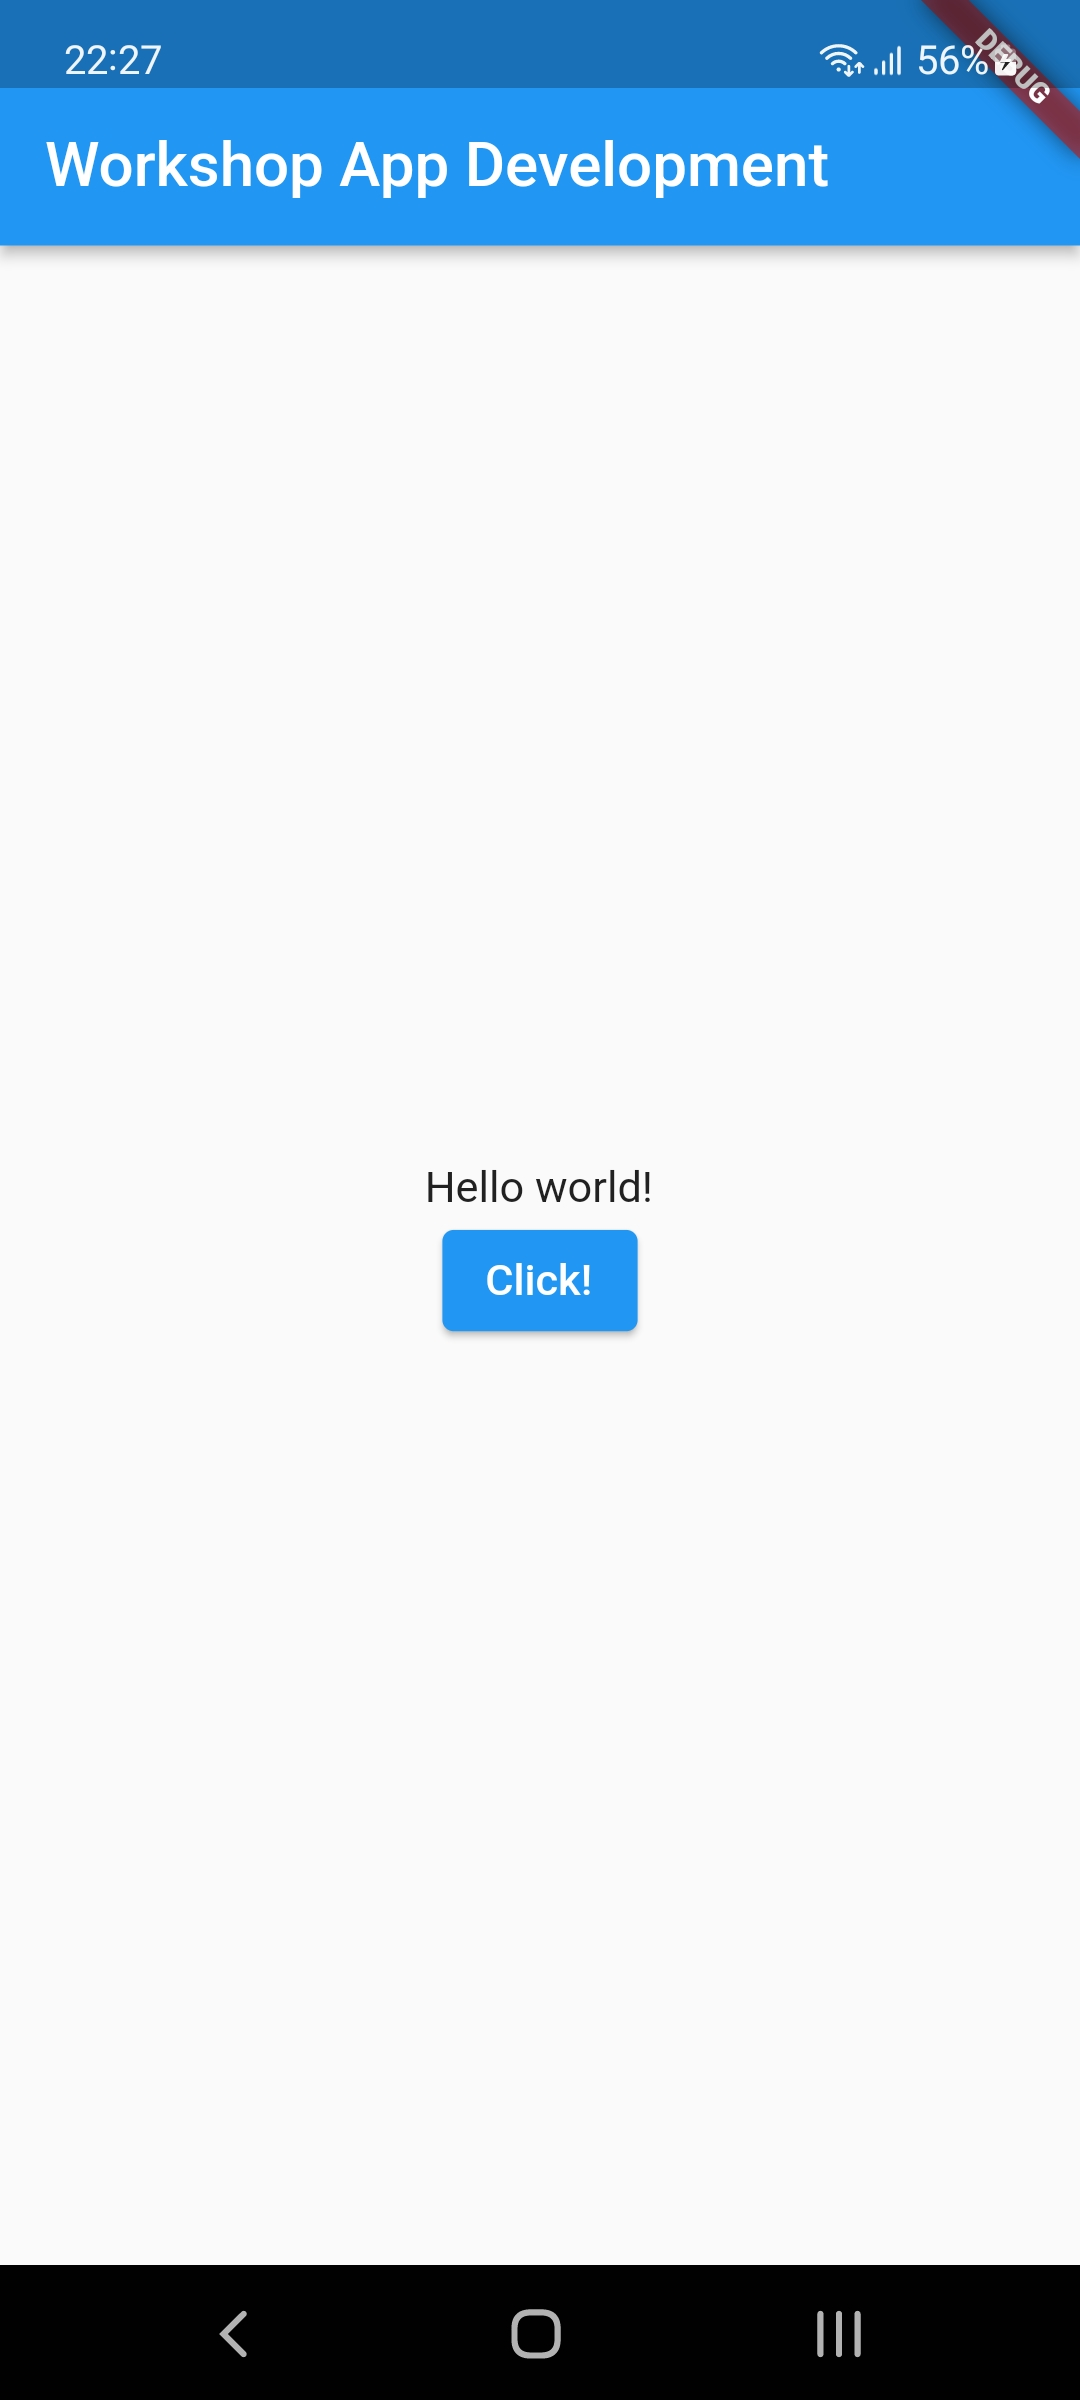
\includegraphics[width=0.3\textwidth]{images/task1.jpg}}
        }
    \end{figure}
\end{frame}

\begin{frame}{Task 1 - Basic Layout}
    \begin{figure}[h]
        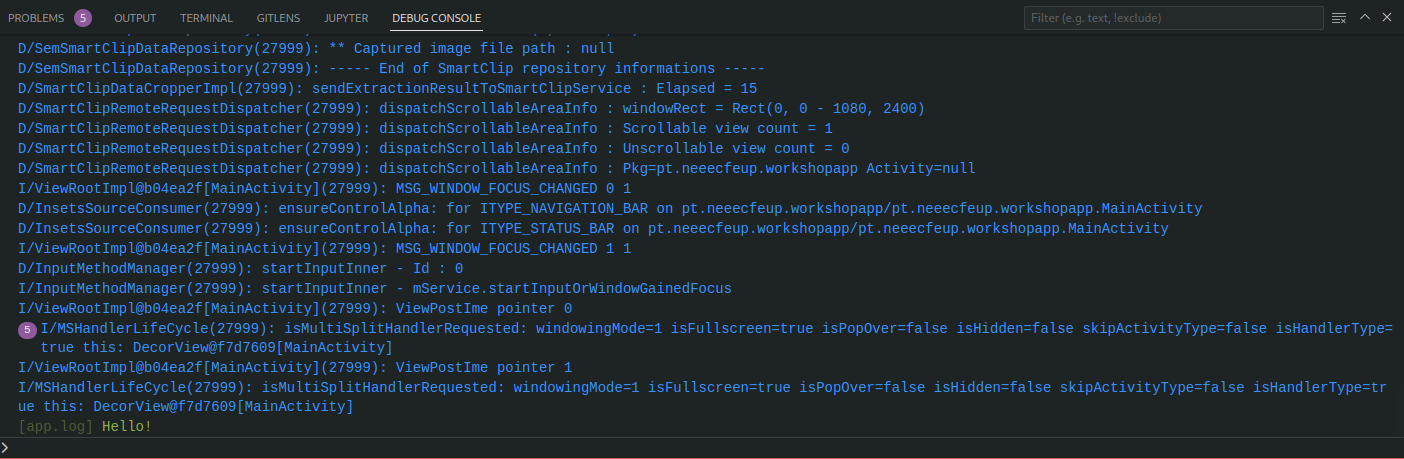
\includegraphics[width=1\textwidth]{images/task1-term.png}
    \end{figure}
\end{frame}

\begin{frame}{References}
  [1] Google, “Flutter documentation.” \url{https://docs.flutter.dev/} (last accessed Nov. 04, 2022).
\end{frame}

{
  \logo{
\includegraphics[height=1.5cm]{images/logo_oficial_branco_c.png}}
  \begin{frame}[standout]
    Questions?
  \end{frame}
}


\end{document}